\section{The Hjj tagger}\label{sec:Hjjtagger}
In this section we introduce a discriminator aiming at identifying a dijet pair that originates from a Higgs decaying to two Ws.
This discriminator represents a possible extension of the Hj tagger described in Sec. \ref{sec:Hjtagger}.
We describe it below for completeness, despite we have not found any direct improvement by using it in the main analysis.

We target the 2lss category in which the ttH signal decays, in the highest fraction of events, according to the following chain:
$$(t) (t) (H) \rightarrow  (bW) (bW) (WW^*) \rightarrow (bjj)  (b\ell\nu_{\ell}) (\ell\nu_{\ell}jj)$$
We therefore expect 2 b quark jets, 4 jets, 2 same-sign leptons, and missing energy in the final state,
altough, in order to increase the signal acceptance, the analysis requires the presence of at least 4 jets overall.
This means that the Higgs jets do not necessarily enter the signal region.

In order to deal with both the complicated jet combinatoric and the possibility that not all the jets originating from Higgs are selected,
a dedicated tagger is developed: the Higgs-dijet (Hjj) tagger.
The Hjj tagger is a discriminator that considers geometric and kinematic features in order to estimate the 
likelihood of a jet pair originating again from $H \rightarrow WW^* \rightarrow \ell\nu_{\ell}jj$.

The discriminator is developed considering the BDT  multivariate technique.
We rely on the powheg ttH sample and ttV sample to define the signal and the background in the training.
For the Hjj tagger the signal is represented by a reconstructed dijet pair that is matched at gen-level to the dijet pair
of the process $H \rightarrow WW^* \rightarrow \ell\nu_{\ell}jj$, while the background is given by the reconstructed dijet pairs in the ttV events.
For the training, we consider the phase space of events that enter the 2lss category, with 0 $\tau_h$.

In the following subsection we list the variables used for the Hjj tagger and their expected BDT distributions.

\subsection*{Hjj variables and performance}
The variables used for the Hjj tagger are:
\begin{itemize}
\item sum of the Hj taggers for the two jets 
\item dR of the two jets
\item minimum dR between the jet pair and another jet
\item ratio of the minimum and maximum dR between the jet pair and another jet
\item dijet mass
\item mass of the dijet plus the closest lepton
\end{itemize}

The performances of the Hjj tagger are illustrated in Fig. \ref{fig:HjjDistrROC}.

\begin{figure}[htb]
 \centering
   %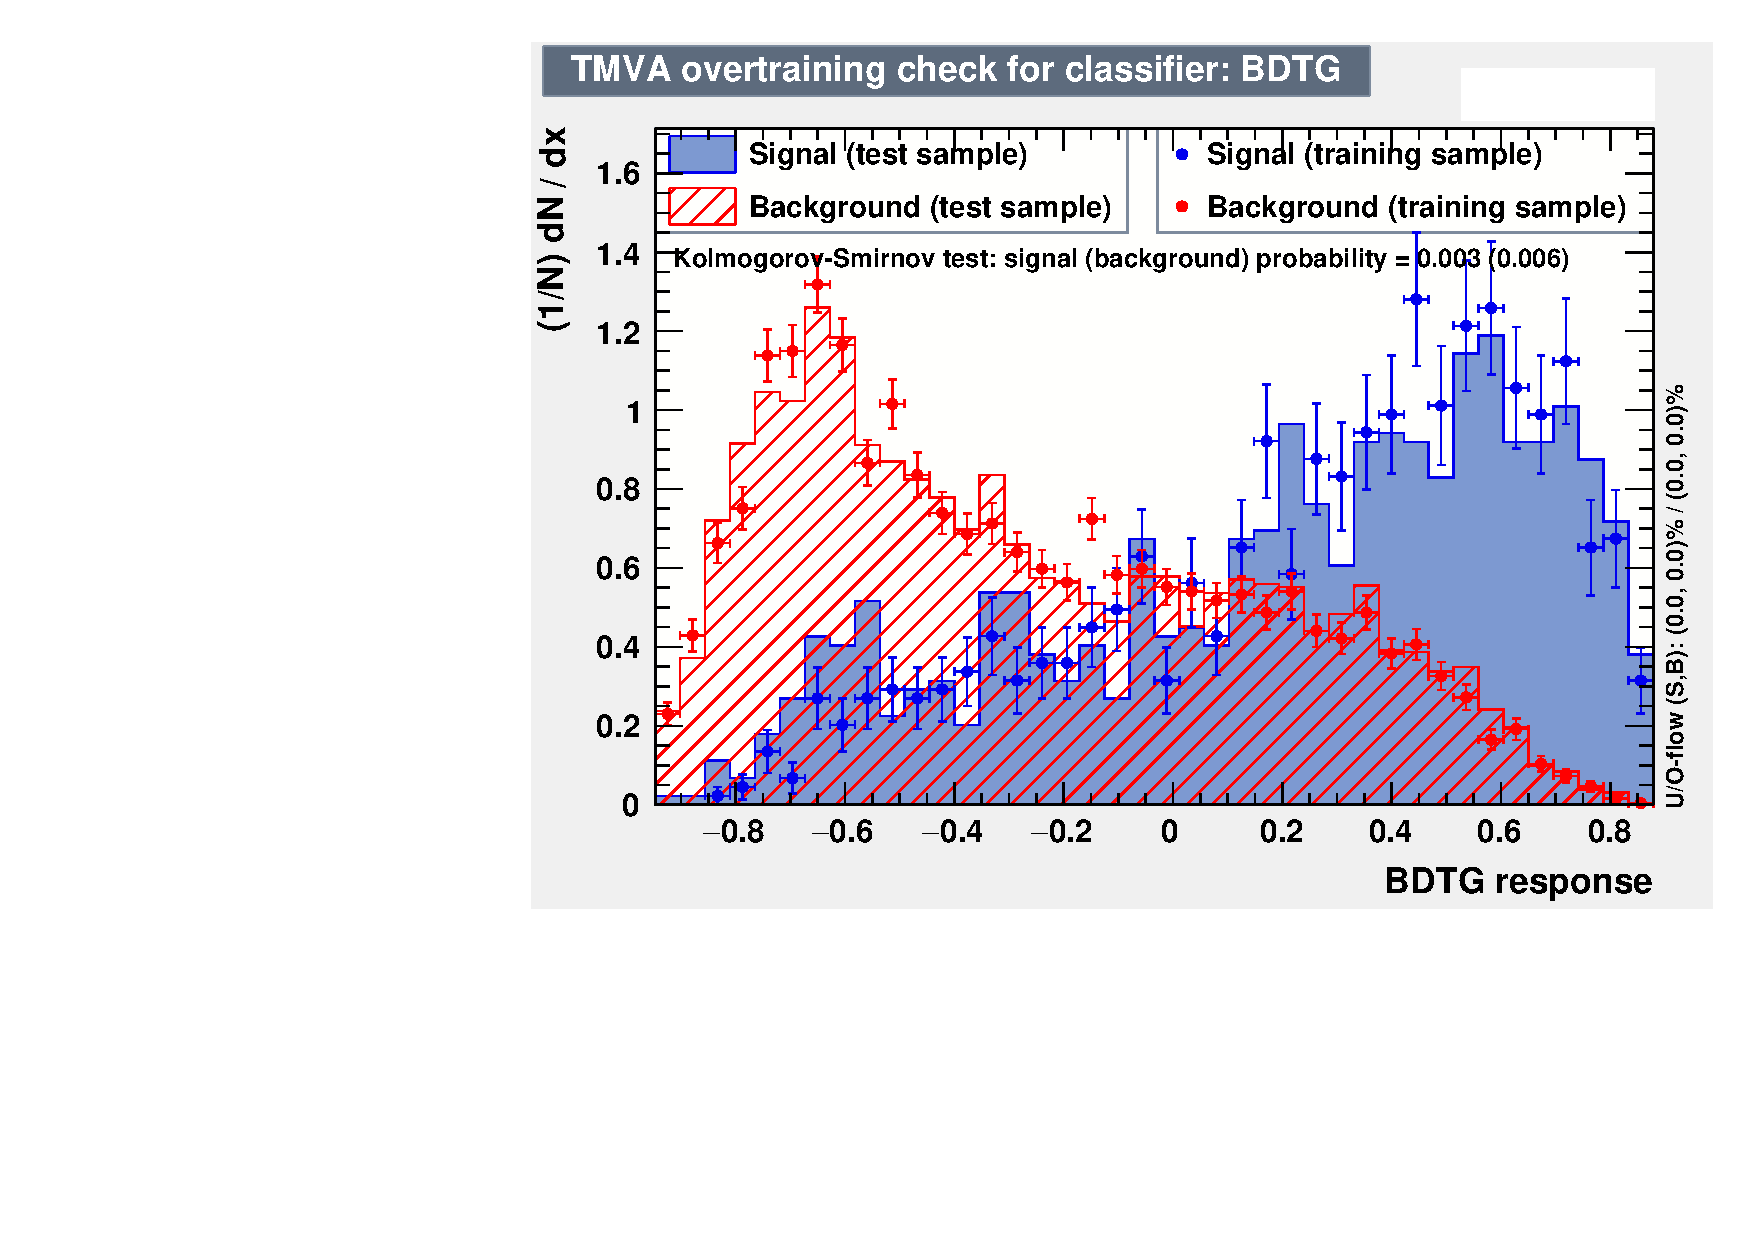
\includegraphics[width=0.48\textwidth]{plots_HjHjj/JJtagger_Ks.pdf}
   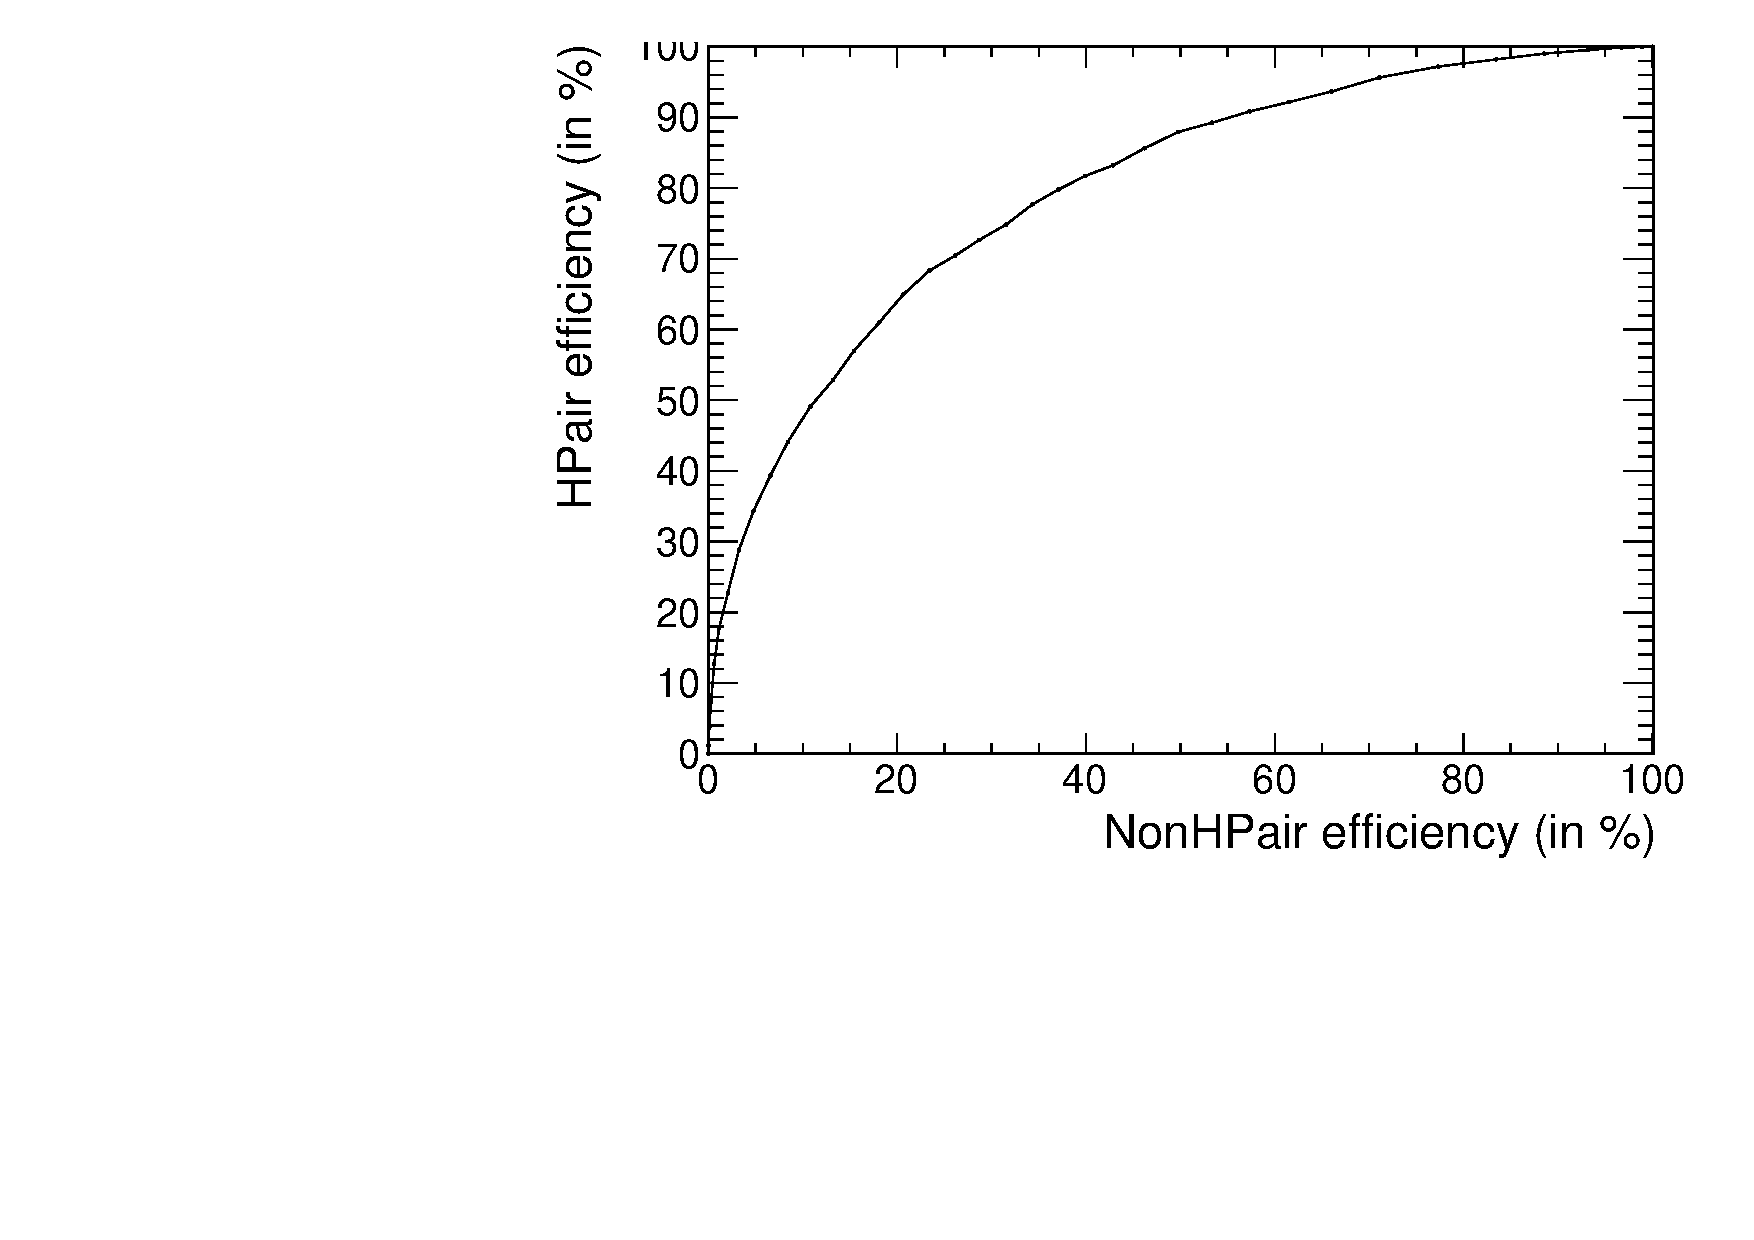
\includegraphics[width=0.48\textwidth]{plots_HjHjj/JetPair_30Jan.pdf}
   \caption{The Hjj ROC. Signal and background composition are described in the text.}
   %\caption{The Hjj distribution (left) and ROC (right). Signal and background composition are described in the text.}
  \label{fig:HjjDistrROC}
\end{figure}
